\section{Généralités sur le cerveau}

Pour mieux comprendre l'aphasie en général et celle de Broca en particulier, 
il convient de commencer avec le cerveau.
Il s'agit du système biologique le plus complexe connu~\cite{}.
Avec le cervelet et le tronc cérébral, il forme l'encéphale (voir Figure~\ref{fig:brain}).
Le cerveau se charge du traitement des flux nerveux sensoriels et moteurs.
Il est aussi le siège des hautes fonctions cognitives comme l'inférence logique, l'émotion 
et --- crucialement pour notre étude --- le traitement du langage.

\begin{figure}[htb]
    \begin{center}
        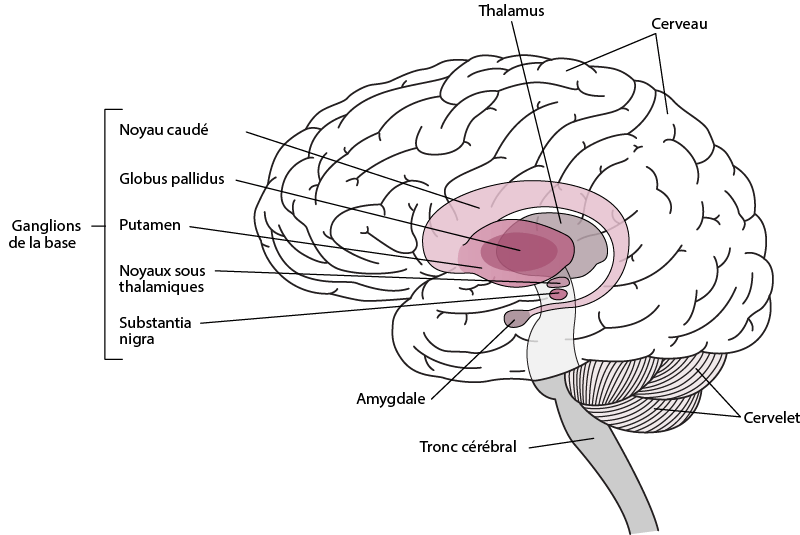
\includegraphics[width=.8\textwidth]{brain.png}
    \end{center}
    \caption{Encéphale humain}
    \label{fig:brain}
\end{figure}

Le cerveau est composé de deux hémisphères ; chacun desquels se divise en lobes : 
frontal, temporal, pariétal et occipital (voir Figure~\ref{fig:lobes}).
La surface du cerveau s'appelle le ``cortex cérébral''.
Il présente plusieurs circonvolutions qui augmentent considérablement sa surface.
Le cortex cérébral est divisé en régions fonctionnelles qu'on appelle ``aires'' 
(voir Figure~\ref{fig:brain-areas}).
Le travail de Dr.~Broca sur le cas de M.~Leborgne est largement reconnu comme l'origine de cette division.


\begin{figure*}[htb]
    \begin{center}
        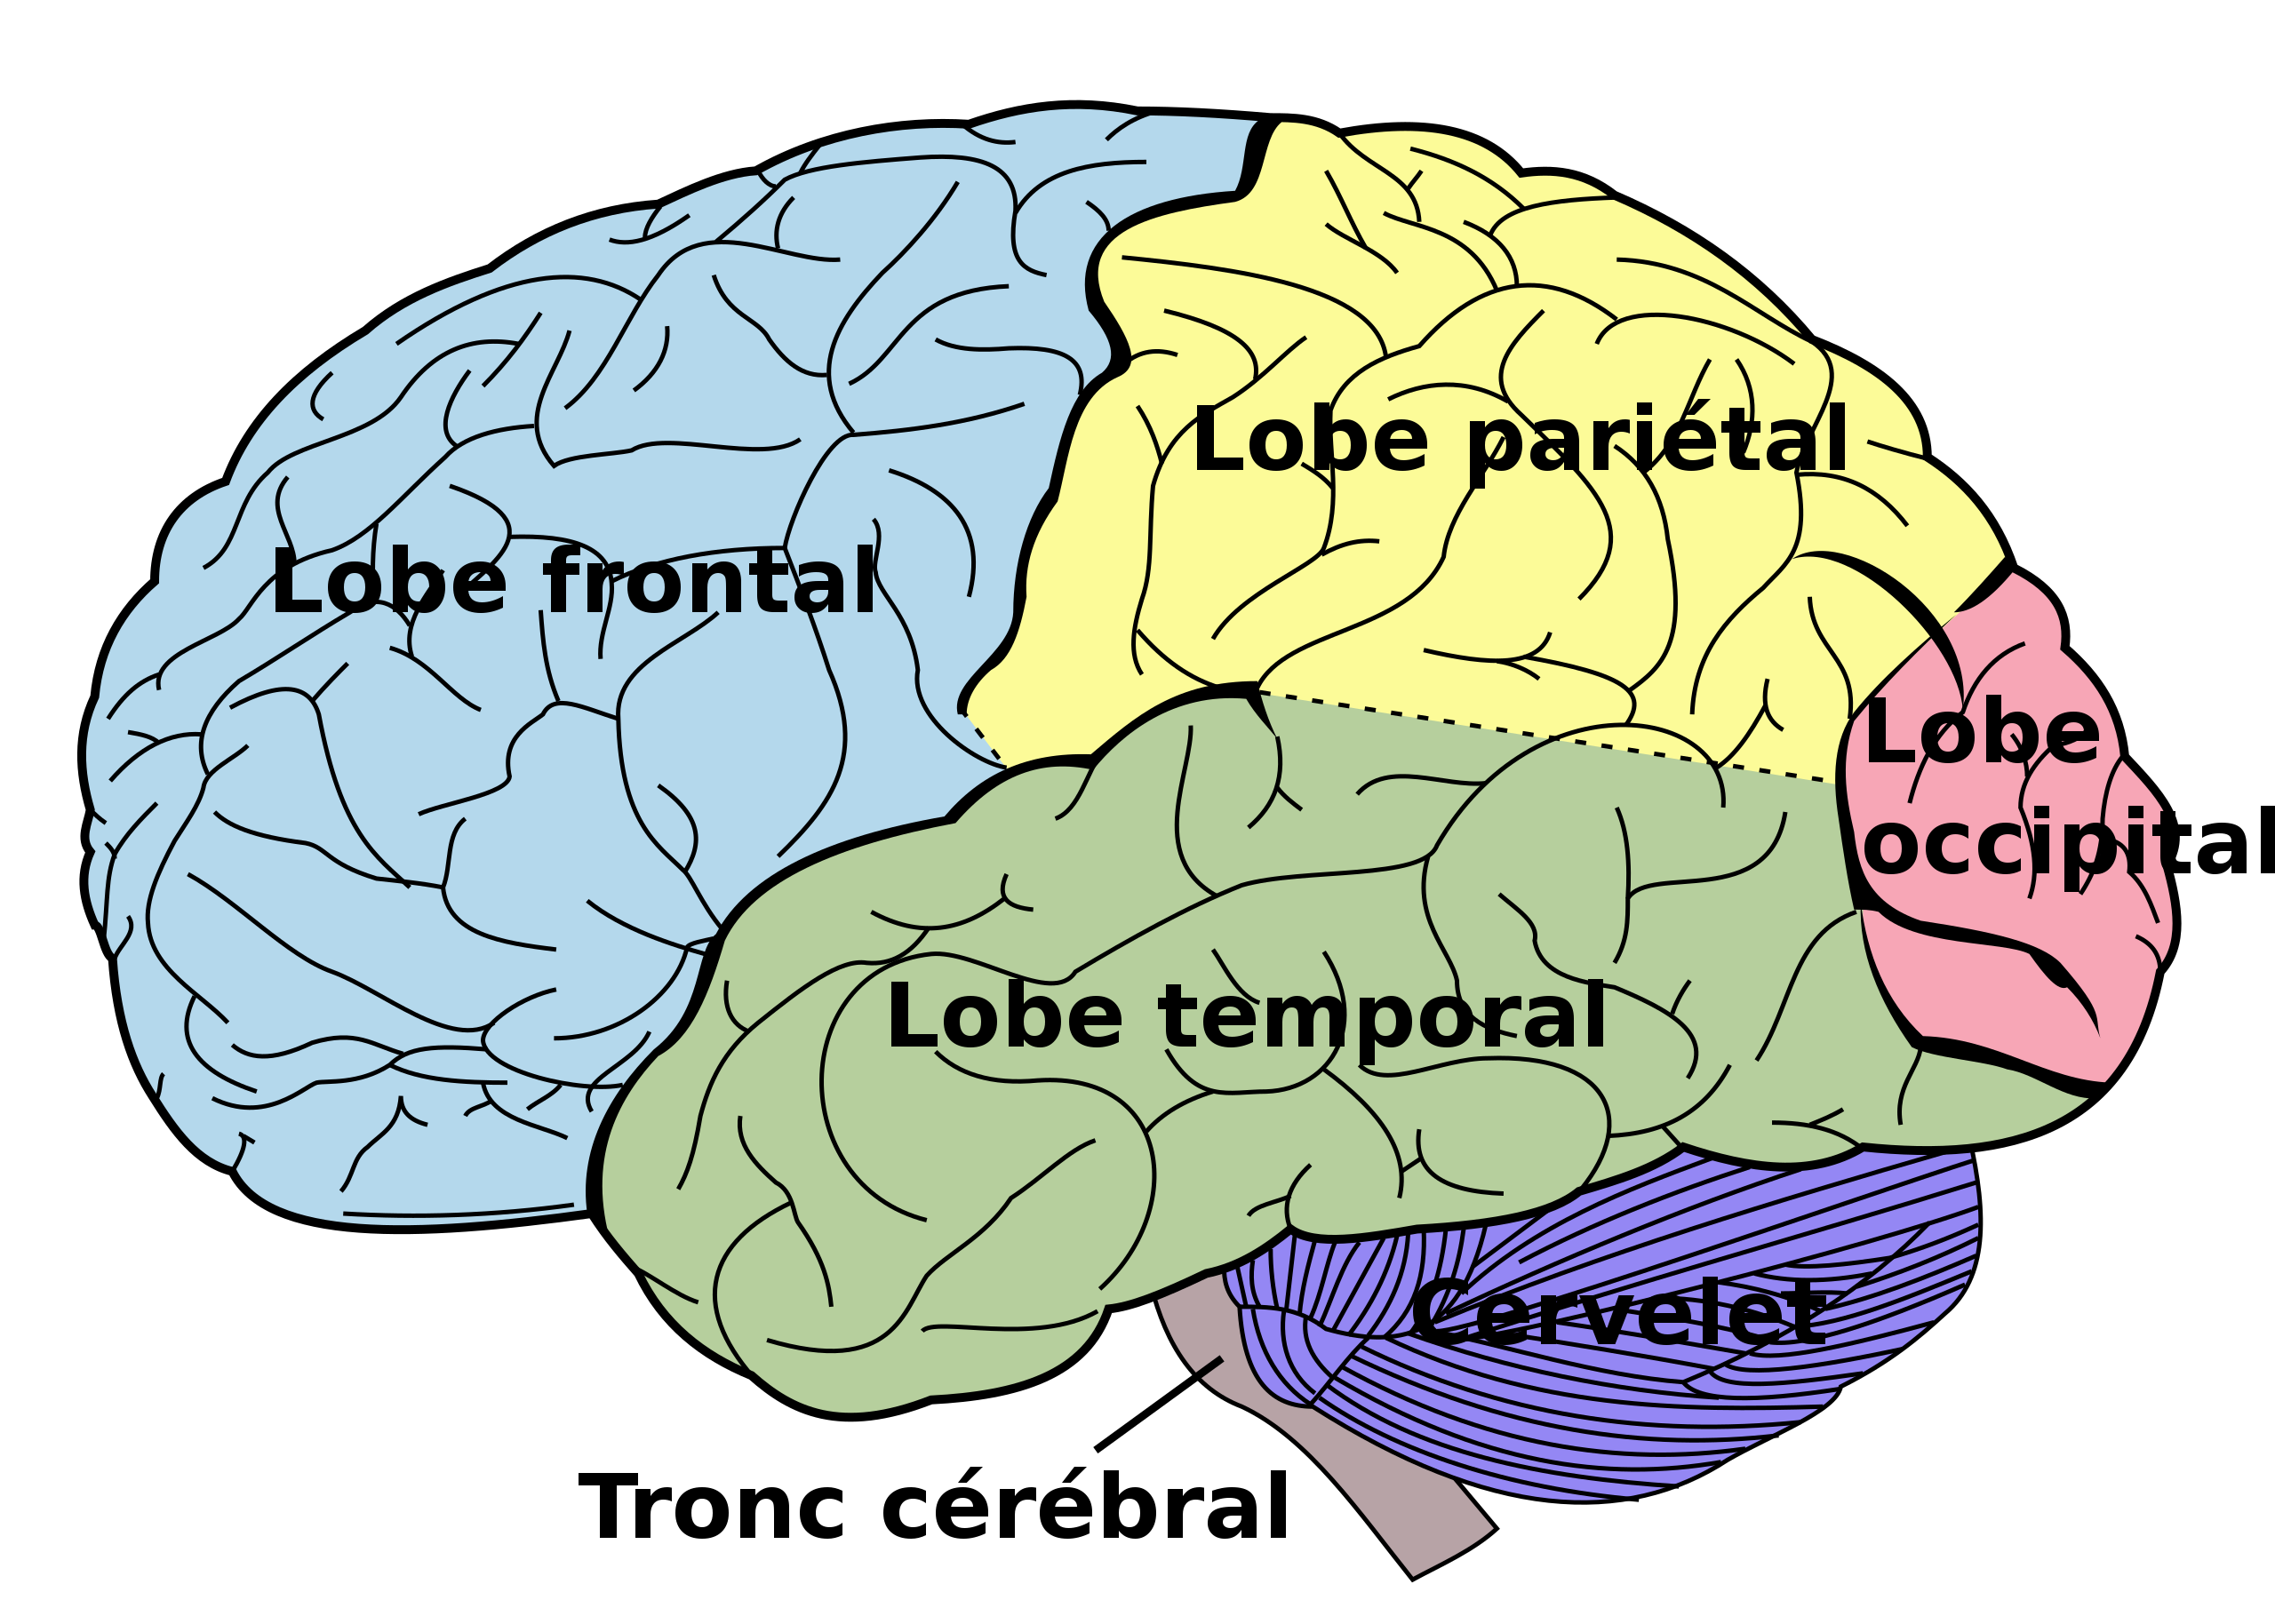
\includegraphics[width=10cm]{lobes.png}
    \end{center}
    \caption{Lobes du cerveau}
    \label{fig:lobes}
\end{figure*}

\begin{figure}[htb]
    \begin{center}
        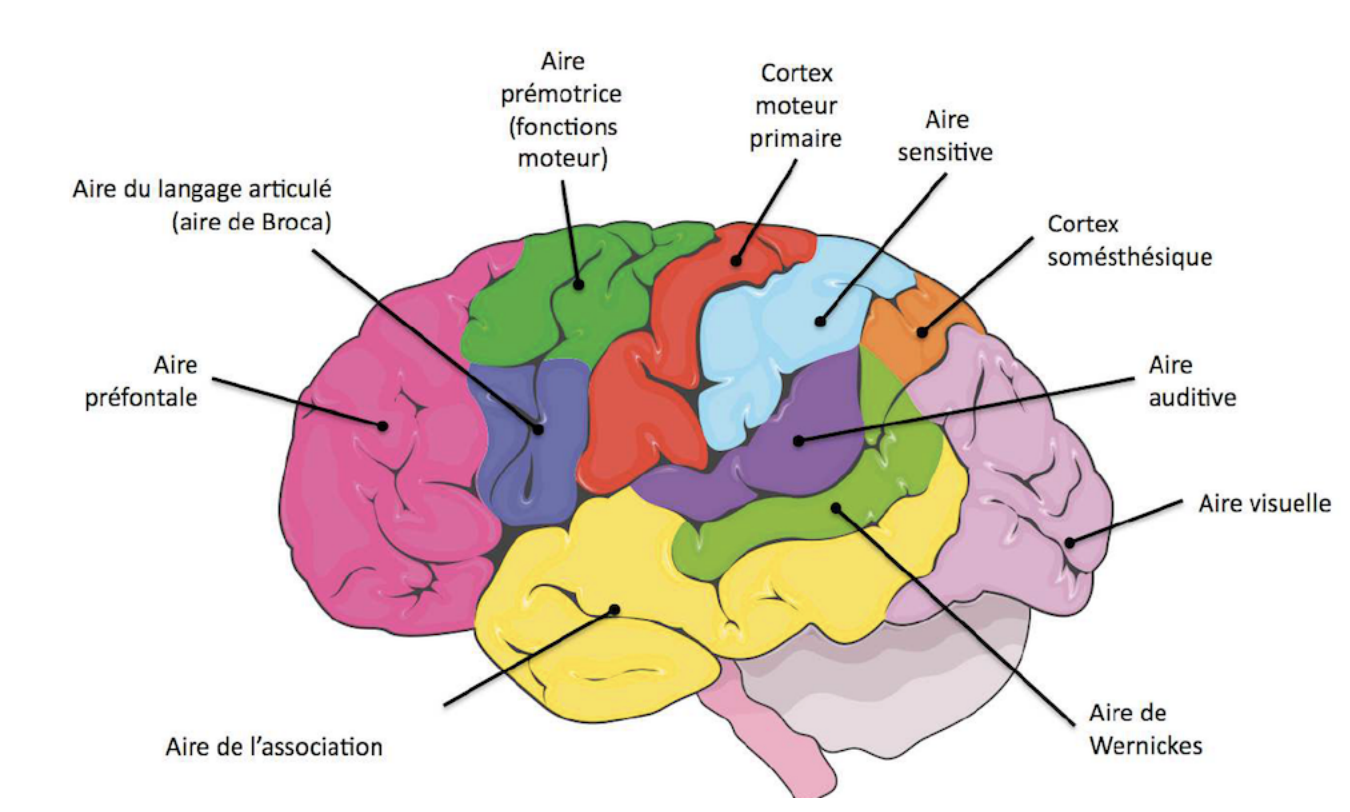
\includegraphics[width=10cm]{areas.png}
    \end{center}
    \caption{Aires du cortex cérébral}
    \label{fig:brain-areas}
\end{figure}